% PROTOKOLL Action Item
\documentclass[
   draft=false
  ,paper=a4
  ,twoside=false
  ,fontsize=11pt
  ,headsepline
  ,DIV11
  ,parskip=full+
]{scrartcl} % copied from Thesis Template from HAW

\usepackage[ngerman,english]{babel}
\usepackage[T1]{fontenc}
\usepackage[utf8]{inputenc}

\usepackage[
    left  =4em
   ,right =4em
   ,top   =5em
   ,bottom=5em
]{geometry}

\usepackage{longtable}
\usepackage[german,refpage]{nomencl}

\usepackage{float}
\usepackage{enumitem}
\usepackage{hyperref} % for a better experience

\hypersetup{
   colorlinks=true % if false - links get colored frames
  ,linkcolor=black % color of tex intern links
  ,urlcolor=blue   % color of url links
}

\usepackage{graphicx}
\usepackage{amsmath}

\usepackage{array}   % for \newcolumntype macro
\newcolumntype{L}{>{$}l<{$}} % math-mode version of "l" column type
\newcolumntype{R}{>{$}r<{$}} % math-mode version of "r" column type
\newcolumntype{C}{>{$}c<{$}} % math-mode version of "c" column type

\usepackage{listing}
\usepackage{caption}
\usepackage{colortbl}
\definecolor{tabgrey}{rgb}{0.85,0.85,0.85}
%using minted because of the hashtag in bash

\sloppy
\clubpenalty=10000
\widowpenalty=10000
\displaywidowpenalty=10000

\begin{document}

\selectlanguage{ngerman}
% ----------------------------------------------------------------------------
% ---------------------------------------------------------- HIER WAS MACHEN -
% -------------------------------- Metadaten wie namen und Gruppentreffen etc-
\def\titel{AD Praktikum: Aufgabe 04, Pascals Dreieck}


\def\teilnehmer{ 
	& Martin Witte & \\
    & Karl-Fabian Witte   & \\
}
% -------------------------------------------------- HIER AUFHÖREN ----------




% ------------------------------------------ einige strukturell Definitionen
\newlength{\txtw} %definiere neue länge
\setlength{\txtw}{\textwidth} %setze neue länge auf textbreite
\addtolength{\txtw}{-10\tabcolsep} %subtrahiere -8\cdot textbreite von asdf

\def\me{\myName \newline \footnotesize{\url{\myEmail} } }

% ------------------------------------------------------------------ Inhalt	
\begin{tabular}{l p{0.4\txtw} p{0.4\txtw} }
	\teilnehmer
	& & \\
	& \today & \\
\end{tabular}

\section*{Abstract}
\centering
Die Berechnung des Pascal`sche Dreieck soll in drei verschiedenen Algorithmen realisiert werden. Die \mbox{Komplexität} der Implementationen soll mittels einer Messung bestimmt werden. Die Algorithmen wurden rekursiv, iterativ und über den Binominalkoeffizienten für natürliche Zahlen realisiert.  

\normalsize
\subsection*{Methoden}

\subsubsection*{1. Rekursive-Methode}
In der rekursiven Methode wird die N'te Zeile des Pascal`schen Dreiecks von der 0'ten Zeile an, Zeile für Zeile, durch Wiederaufrufen der gleichen Funktion errechnet.
$ $

\subsubsection*{2. Iterative-Methode}
In der iterativen Methode wird die N'te Zeile des Pascal`schen Dreiecks von der 0'ten Zeile an, Zeile für Zeile, durch N-fachen Schleifenaufruf berechnet.
$ $

\subsubsection*{3. Binominalkoeffizient-Methode}
In der Binominalkoeffizient-Methode hier, FastPascal genannt, wird die N`te Zeile des Pascal`schen Dreiecks, direkt, mit Hilfe der Formel 
$\binom{n}{k} = \frac{n!}{k!*(n-k)!}$ 
für jede 'Spalte' der Zeile berechnet.
Aufwand: $(\sum\nolimits_{k=1}^{N-1})+(\sum\nolimits_{k=1}^{N-1}) = 2N$


\flushleft
\subsection*{Die Messung}
	
\begin{figure}[htp]
	\label{fig:recuriterfast}
  	\centering
    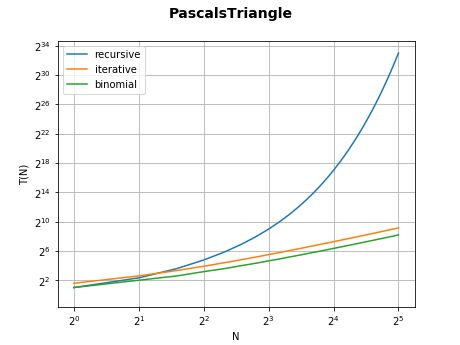
\includegraphics[width=\textwidth]{./IMG/PascalsTriangle.png}
    \caption[recur iter fast]{Die Aufwende der Implementationen des rekursiven, iterativen und die über den Binomialkooeffizienten Algorithmen sind gegen die Dreieckstiefe N aufgetragen.}
\end{figure}
	
\begin{figure}[htp]
	\label{fig:iterfast}
  	\centering
    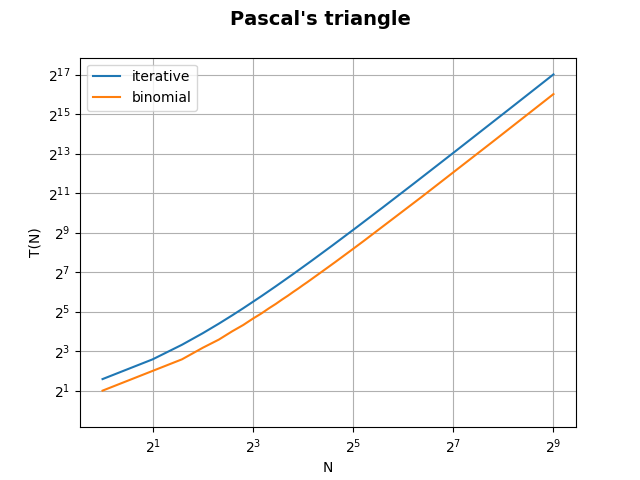
\includegraphics[width=\textwidth]{./IMG/iterfast.png}
    \caption[iter fast]{Die Aufwende des iterativen und die angeblich schnellere Implementation über den Binomialkooeffizienten sind gegen die Dreieckstiefe N aufgetragen.}
\end{figure}




\end{document}
% vim: set spell spelllang=de :EOF
